% !TeX spellcheck = en_US 
\documentclass[11pt]{article}

\usepackage{amssymb} % see: http://milde.users.sourceforge.net/LUCR/Math/mathpackages/amssymb-symbols.pdf
\usepackage{mathtools} % for extended mathematical symbols and more

% Page properties :
% See : https://tex.stackexchange.com/questions/36085/latex-without-pages
\usepackage{geometry}
\geometry{margin=16mm}

\usepackage{caption}


% fix for underlined text not hyphenating :
%\usepackage{soul} % use this
% then replace '\underline{}' with '\ul{}'

% To color text :
% see : https://en.wikibooks.org/wiki/LaTeX/Colors
\usepackage[dvipsnames]{xcolor} % use this
% then use one of these syntaxes :
% >\textcolor{declared-color}{text}
% >{\color{declared-color} text}

% Input file encoding :
\usepackage[utf8]{inputenc}     % makes accents not shit

% To use images : 
\usepackage{graphicx} % use this
\graphicspath{ {./IMG/} } % path midifier for storing images
% to include a picture, type this ('name' is without path or extention) :
% \includegraphics[width=0.5\textwidth]{name}

% Box : % width should be manually set
% \fbox{ \parbox{0.8\textwidth}{ text } }

% Espacement :
% \hfill \vfill
% \vspace{length} \hspace{length} % if ignored, use starred version or { \vspace*{length} }
% \phantom{text} 
% Indentation explicite :
% \indent et \noindent
\usepackage{parskip}

% Fractions :
% \frac{num}{denum}  % small text num/denum
% \dfrac{num}{denum} % normal text num/denum

% Coloring text: % works on text and math modes
% \textcolor{declared-color}{text}
% {\color{declared-color}some text}

% How to use references :
\usepackage{hyperref} % use this
% use '\hypertarget{some_label}{}', then
% and reference it with '\hyperlink{some_label}{some text}'
\hypersetup{
	colorlinks=true,    
	urlcolor=blue,
}

% To write prooftrees :
% see : http://www.pirbot.com/mirrors/ctan/macros/latex/contrib/ebproof/ebproof.pdf
%\usepackage{ebproof} % use this


% Verbatim blocks :
\usepackage{verbatim} % normal verbatim
\usepackage{fancyvrb} % for fancy boxed varbatims
\usepackage{parskip}

% For code
\usepackage{listings}
%\begin{lstlisting}
%Put your code he<re.
%\end{lstlisting}


\usepackage{color}

\definecolor{mylightgray}{rgb}{0.95,0.95,0.95}
\definecolor{mygreen}{rgb}{0,0.6,0}
\definecolor{mygray}{rgb}{0.5,0.5,0.5}
\definecolor{mymauve}{rgb}{0.58,0,0.82}

\usepackage[super]{nth}

% Regulates \tableofcontents max depth
\setcounter{tocdepth}{2}

\usepackage{array}
\newcolumntype{L}[1]{>{\raggedright\let\newline\\\arraybackslash\hspace{0pt}}m{#1}}
\newcolumntype{C}[1]{>{\centering\let\newline\\\arraybackslash\hspace{0pt}}m{#1}}
\newcolumntype{R}[1]{>{\raggedleft\let\newline\\\arraybackslash\hspace{0pt}}m{#1}}

\usepackage{xcolor,colortbl}
\newcolumntype{a}{>{\columncolor{mylightgray}}l}

\usepackage{array}
\setlength\extrarowheight{4pt} % or whatever amount is appropriate

\lstset{ 
	backgroundcolor=\color{mylightgray},   % choose the background color; you must add \usepackage{color} or \usepackage{xcolor}; should come as last argument
	basicstyle=\small,        % the size of the fonts that are used for the code
	breakatwhitespace=false,         % sets if automatic breaks should only happen at whitespace
	breaklines=true,                 % sets automatic line breaking
	captionpos=b,                    % sets the caption-position to bottom
	commentstyle=\color{mygreen},    % comment style
	deletekeywords={...},            % if you want to delete keywords from the given language
	escapeinside={\%*}{*)},          % if you want to add LaTeX within your code
	extendedchars=true,              % lets you use non-ASCII characters; for 8-bits encodings only, does not work with UTF-8
	firstnumber=1,                % start line enumeration with line 1000
	frame=single,	                   % adds a frame around the code
	keepspaces=true,                 % keeps spaces in text, useful for keeping indentation of code (possibly needs columns=flexible)
	keywordstyle=\color{blue},       % keyword style
	%language=Java,                 % the language of the code
	morekeywords={},            % if you want to add more keywords to the set
	numbers=none,                    % where to put the line-numbers; possible values are (none, left, right)
	numbersep=5pt,                   % how far the line-numbers are from the code
	numberstyle=\tiny\color{mygray}, % the style that is used for the line-numbers
	rulecolor=\color{black},         % if not set, the frame-color may be changed on line-breaks within not-black text (e.g. comments (green here))
	showspaces=false,                % show spaces everywhere adding particular underscores; it overrides 'showstringspaces'
	showstringspaces=false,          % underline spaces within strings only
	showtabs=false,                  % show tabs within strings adding particular underscores
	stepnumber=2,                    % the step between two line-numbers. If it's 1, each line will be numbered
	stringstyle=\color{mygreen},     % string literal style
	tabsize=2,	                   % sets default tabsize to 2 spaces
	title=\lstname                   % show the filename of files included with \lstinputlisting; also try caption instead of title
}
\usepackage[english]{babel}
\usepackage{lipsum}
\usepackage{multirow,booktabs} % https://jdhao.github.io/2019/08/27/latex_table_with_booktabs/

\newcounter{codeID}[section]
\newcommand{\nextcodeID}{\refstepcounter{codeID}\multirow{3}{*}{\thecodeID}}

\usepackage{longtable}

\newcommand{\degrees}[1]{#1$^{\circ}$}

\usepackage{pgfplots, tikz}


%opening
\title{Pokemon Essentials - Extraction}
\author{David Rodriguez Soares}


% first page
\begin{document}
\maketitle

\vspace*{\fill}

\textbf{Privacy policy}

This is a confidential document and should not be distributed under any circumstance. \hyperref[sec:privacypolice]{Please click and read}.

\vspace{20mm}

\newpage

\begingroup
\hypersetup{linkcolor=black}
\tableofcontents
\endgroup

\newpage
\section{What this document is about}

This document holds information about how to extract Pokemon Essentials game data, which is relevant in project PoGER's goal of proposing an implementation free from RPG Maker XP.

Please read this document's \hyperref[sec:privacypolice]{Privacy Policy}.

As a result of the limited scope of PoGER and the limited time and information available to the author, the following documentation isn't complete and may not be accurate.

The information was obtained through the official RPG Maker XP built-in documentation, user content found on the internet (forum posts, videos) and the author's reverse-engineering work.

The following abbreviations may be present :
\begin{itemize}
	\item \textbf{RMXP} - RPG Maker XP
	\item \textbf{PE} - Pokemon Essentials
	\item \textbf{RGSS} - Ruby Game Scripting System
\end{itemize}

Please note that the author is not a native English speaker.


\subsection{Reminder - PoGER and motivations}

PoGER is an academic research project, that started as an interest to understand of how Pokemon Essentials (and its derived games) work.

What I rapidly determined was that tools like RMXP and PE weren't adapted to creating a game in a \textit{modern} way, and suffered from their age and design decision, to the point that they were basically abandoned and deprecated. It was clear to me that I should not try to build upon them, but rather bring them up somehow.

I started by identifying shortcomings of the studied software, then moved on to coming up with solutions.

I'm looking into implementing a similar engine that would be decoupled from RPG Maker XP  and would run games as programs written in an interpreted domain-specific language I would create. 

This document covers the complementary pieces of software that automate the port of Pokemon Essentials. Games based on PE should be able to be ported through the same process, with perhaps a few tweaks.


\subsection{Reminder - technical findings}

\subsubsection{Structure}

PE and its derivatives share a common project structure :

\begin{tabular}{|r L{.1\linewidth}|L{.8\linewidth}|}
	\hline
	$\circ$ & Root & Contains compiled game files and libraries, plus a few useful programs, some probably made by Pokemon Essentials developers. \\
	\hline
	\rotatebox[origin=c]{180}{$\Lsh$} & Audio & Contains the musical assets of the game, typically MIDI and OGG files. \\
	\hline
	\rotatebox[origin=c]{180}{$\Lsh$} & Data & Contains the logic of the game and most of its data.  \\
	\hline
	\rotatebox[origin=c]{180}{$\Lsh$} & Fonts & Contain fonts used for displaying text. \\
	\hline
	\rotatebox[origin=c]{180}{$\Lsh$} & Graphics & Contains the graphical assets of the game, typically tile sets, in a well organized folder structure. \\
	\hline
	\rotatebox[origin=c]{180}{$\Lsh$} & (\textit{PBS}) & (Facultative) Contains human-readable data to be compiled, like items, species, types, dialogue (and translations), etc. \\
	\hline
\end{tabular}



\newpage
\subsubsection{Data representation}

The data that constitutes a PE project is diverse :

\begin{tabular}{|L{.1\textwidth}|L{.52\textwidth}|L{.3\textwidth}|}
	\hline
	\rowcolor{mylightgray}
	\textbf{Category} & \textbf{Description} & \textbf{Storage} \\
	\hline
	Scripts & Logic of the game, classes, ect & \verb|Scripts.rxdata| file \\
	\hline
	Objects & Files containing sets of class instances, grouped per file & \verb|dat| and \verb|rxdata| files \\
	\hline
	Maps & Contain map representation (incl. events), one per file & \verb|MapXXX.rxdata| \\
	\hline
	Dialogue & Contain dialogue & TODO \\
	\hline
\end{tabular}


\section{Research}

In order to decouple PE from its original code base and RGSS, it became obvious that all useful data had to be extracted from the project.

Since \verb|Audio|, \verb|Graphics| and \verb|Fonts| directories contain already-accessible data, they didn't require any extraction efforts.

See section \textit{Data representation} for categories of data that were identified to need extraction.


\subsection{Scripts}

What I found :
\begin{itemize}
	\item \verb|Scripts.rxdata| is the second largest compiled file of the project, and contains over 120k lines of code.
	
	\item The script is unique : it is divided in named sections (that appear in RMXP's editor on the left hand side) that allow to manage its colossal line count.
	
	\item Like other compiled files, its content are almost impossible to read outside of RMXP.
\end{itemize}

I spent quite a lot of time working on a python script able to decrypt \verb|rxdata| files, and \verb|Scripts.rxdata| in particular, but didn't have much success, so I tried looking elsewhere.

\textbf{Trying something else} : After some more digging, I found a functional utility that was created for the purpose of editing/extracting the scripts from this file : Gemini Editor.

Here are links to \href{https://forum.chaos-project.com/index.php/topic,10420.0.html}{a forum post about it} and \href{https://github.com/terabin/Gemini}{a github repository}.

With it, I was able to extract Pokemon Essentials scripts (see '\verb|PE_scripts|' directory).

It proved invaluable to be able to explore/search the whole script base using a more powerful code editor, saving lots of time from my attempts to create my own scripts to export data.

Note that extracting scripts isn't really useful : the objective is to get away from the RMXP-tied original codebase. It's only useful for the purpose of understanding how RMXP/RGSS/PE work and how features are implemented.


\subsection{Maps and Events}

Maps are essential to games made with RMXP, and a huge portion of the interface is dedicated to them. They contain textures that build the world and events that add elements of behavior to them.

I documented all I could find on maps the events they contain and more in \verb|RMPX_doc|.

\newpage
What I found :
\begin{itemize}
	\item Trying to extract everything from compiled files would require a lot of effort.
	
	\item Creating scripts in RMXP that extract data is way easier.
	
	\item A solid understanding of the Ruby language and classes involved is mandatory.
	
	\item Class declarations can be found in the code and/or in the official documentation with a bit of digging.
\end{itemize}

\vspace{4mm}
Here is a diagram for classes involved in Map/Event/Tileset data extraction.
\begin{figure}[!h]
	\centering
	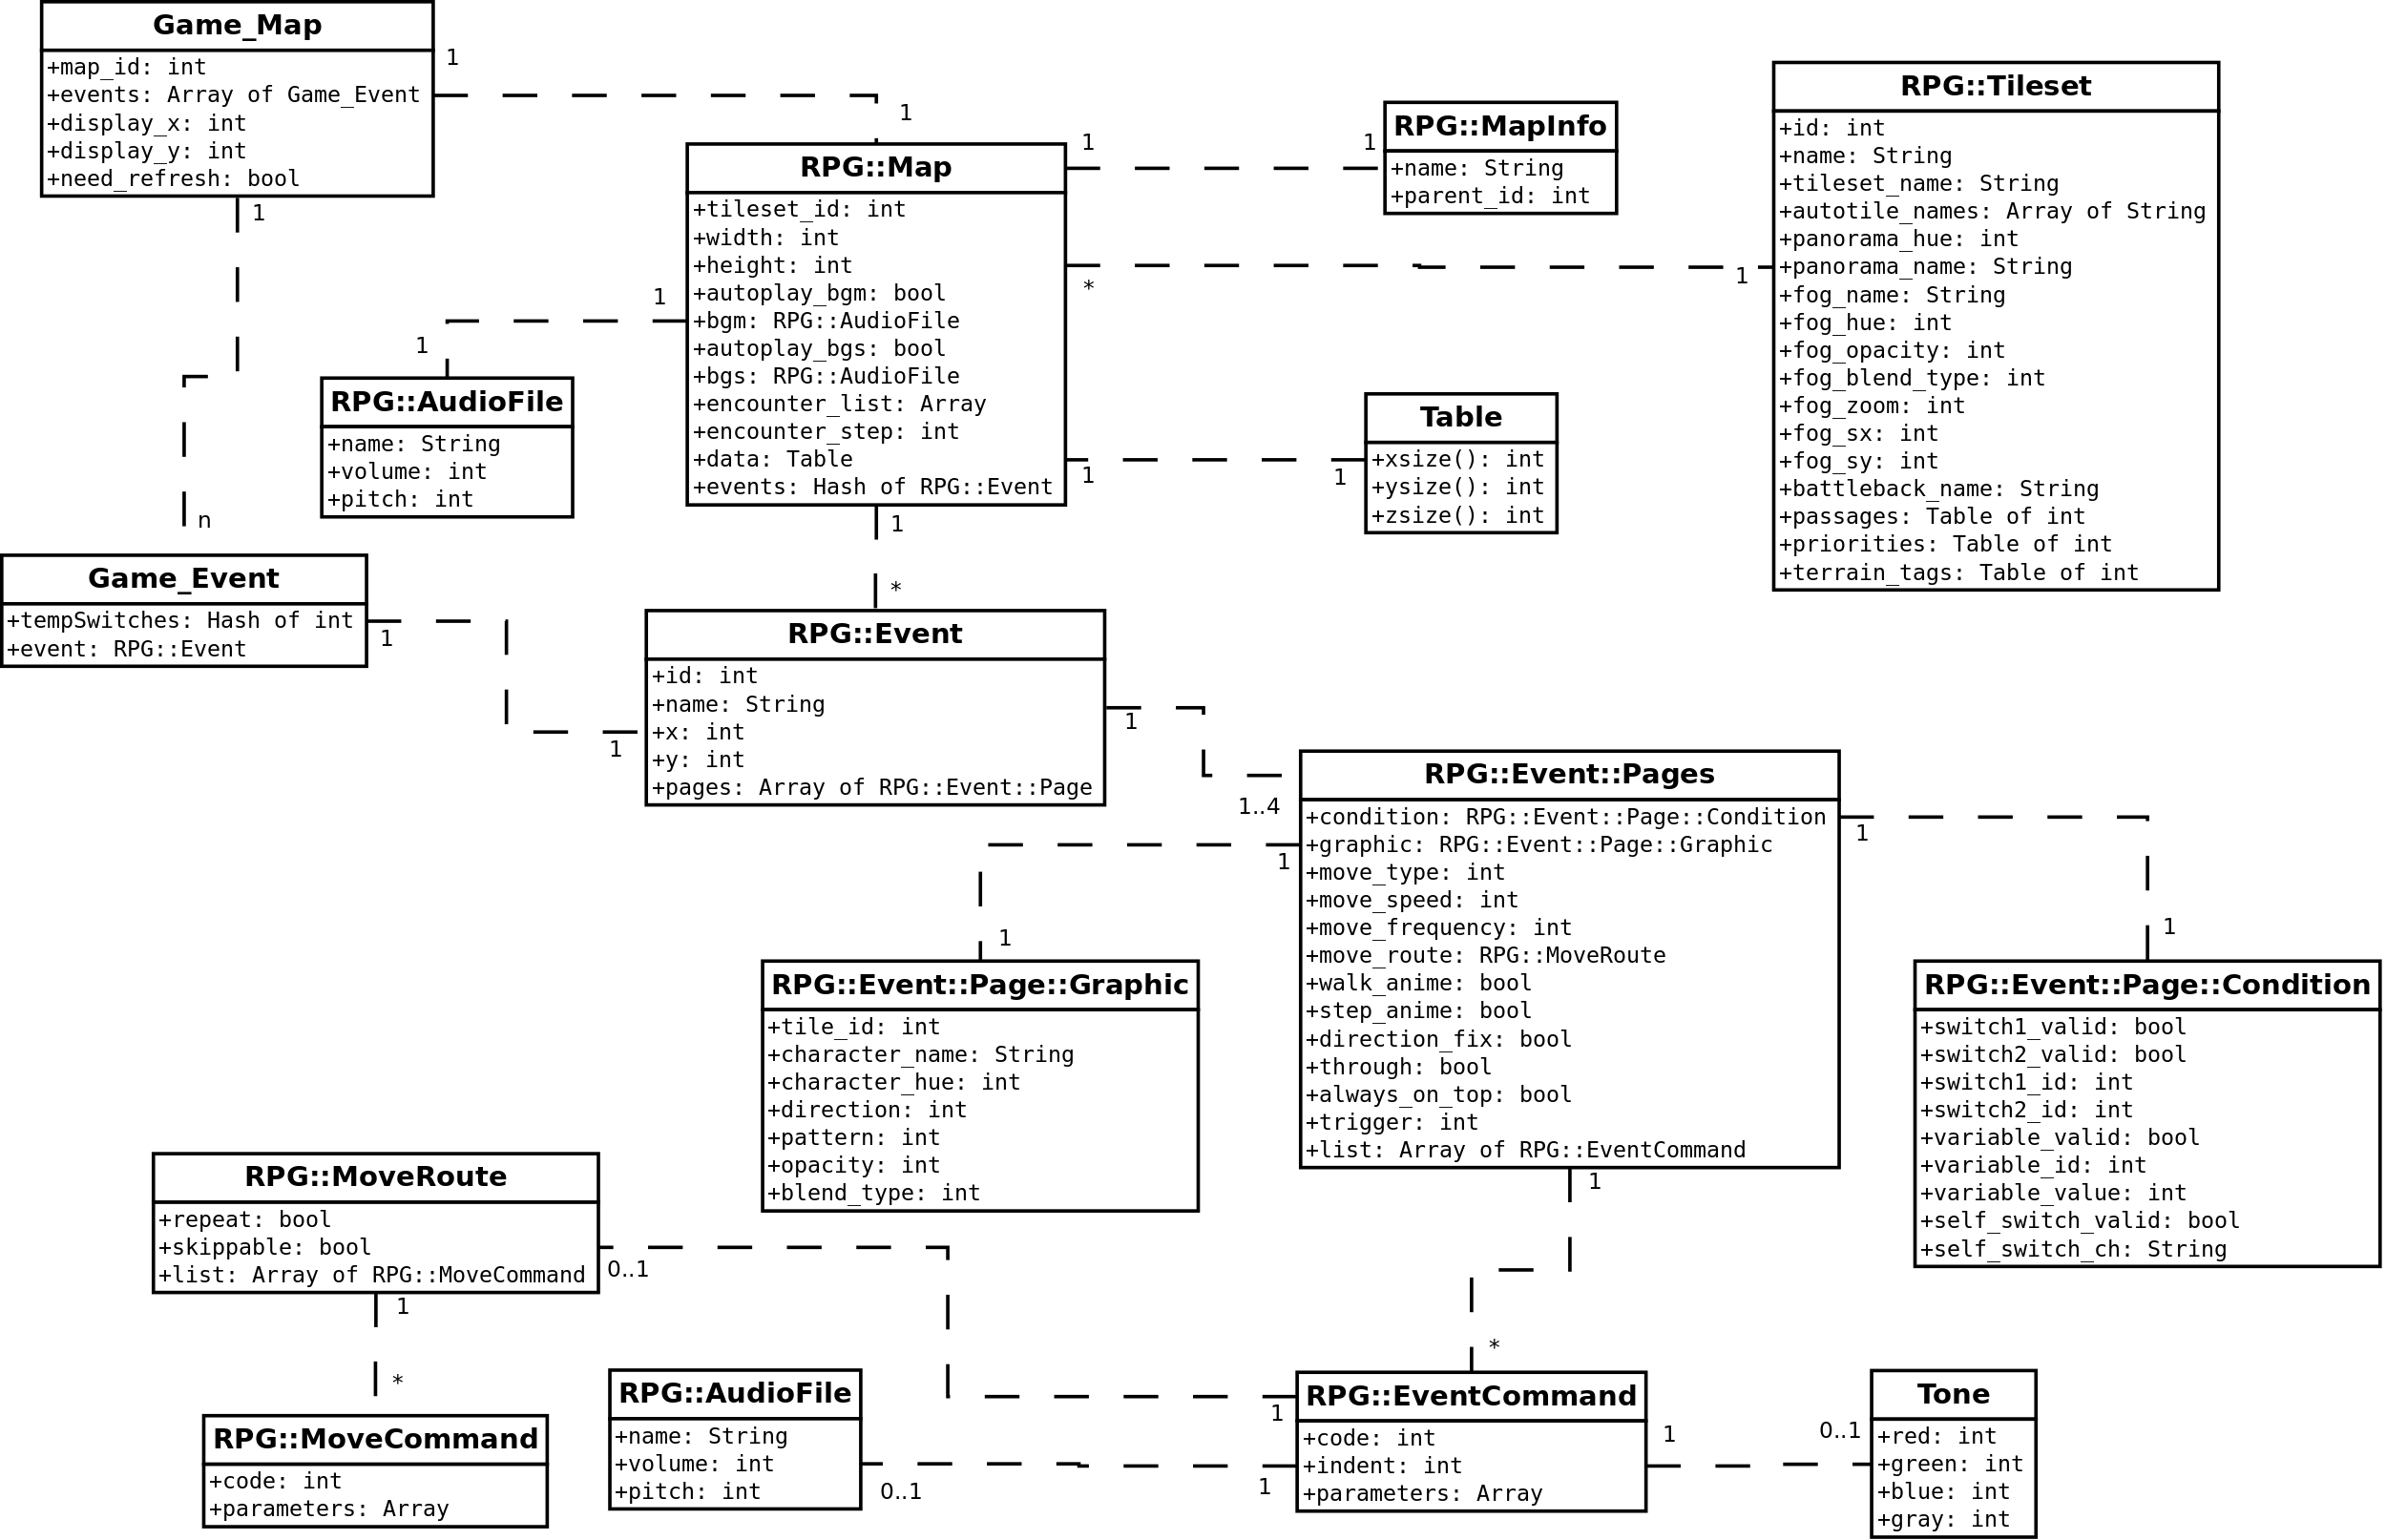
\includegraphics[width=\linewidth]{RMXP_full}
	\caption{Simplified class map representation for Map/Event}
	
\end{figure}


\textit{Semantic/Syntax} : Linked classes (with arity) display an \textbf{associative relationship}.

\textit{Note} : There is no inheritance relationship between any two classes represented. Arities are logically deduced and may not be exact depending in proprietary implementation details. Class \verb|RPG::AudioFile| was duplicated for ease of association routing.


\subsection{Dialogue}

English dialogue is hard-coded in events, therefore in order to propose alternative languages some trickery is needed.

More research is needed here.


\section{Automated extraction process}

Unfortunately, the first steps require the use of RPG Maker XP (version 1.02 tested, other may work also), and therefore Microsoft Windows (XP-10).

It may be possible to run RPG Maker XP on other operating systems using compatibility layers (such as Wine for GNU/Linux), but I didn't try it.

\subsection{Opening a project with RPG Maker XP}

First things first, a copy of the project to extract is needed. It should have the same structure as described in \verb|section 1.2.1|. If so, it should be possible to open it and run it using RPG Maker XP.

Read more about obtaining a copy in \verb|PoGER|.

The following information was obtained through a trial-and-error process when trying to open the Pokemon Essentials and a derivative game (Pokemon Uranium) in RPG Maker XP and run them in order to extract data from them. As such, they may contain erroneous statements or not apply/work for someone else trying to replicate the same process.

\begin{itemize}
	\item You need the following files in the root directory :
	
	\begin{itemize}
		\item \verb|Game.exe| : The executable that launches the game.
		\item \verb|Game.ini| : A configuration file. If the \verb|*.ini| in the project has an other name, \textit{rename a copy} and \textbf{leave the original untouched}, because it seems RMXP needs a \verb|Game.ini| file and game can specify an other name (hard coded in scripts)
		\item \verb|Game.rxproj| : Entry point for RMXP.
		\item \verb|RGSS102E.dll| : Contain RGSS dynamic libraries, probably necessary tu run the executable correctly.
	\end{itemize}

	Renaming files may be needed for some project files.
	
	\item For projects with \textit{compressed data} (no \verb|Data| directory but there is one \verb|*.rgssad| file at root), you need to use an extraction utility.
	
	I used \href{https://gitlab.com/rgss/rgsstool}{RGSS Tool} :
	
	\begin{lstlisting}
	python rgsstool.py -x -d "path\for\output\files" "path\of\rgssad\file"\end{lstlisting}
	\vspace{-8mm}
	
	This worked with Python 3.x, google search it if you're not sure if you have a recent version of Python and how to launch it on your computer.
	
	Exemple for Pokemon Uranium when command line is at root :
	
	\begin{lstlisting}
	python rgsstool.py -x -d . Uranium.rgssad\end{lstlisting}
	\vspace{-6mm}
	
	\item For projects missing the \verb|*.rxproj| file, simply create a new empty file and write the following : 
	
	\fbox{\ttfamily RPGXP 1.02}
	
	Save it with UTF-8 encoding and no "new line" character.
	
	\item Save files should be located in \verb|C:\Users\<user_name>\Saved Games\<name_of_the_game>\|
	
	\item Tip : When running the project from RPG Maker XP, some files in the \verb|Data| directory may be recompiled, which can cause errors. Keep a copy of the content of this directory in case you need to restore its content (you can exclude the \verb|Scripts.rxdata| if you're editing the scripts, so you don't lose progress on this file).
\end{itemize}


\newpage
\subsection{RMXP script}

The first step uses RPG Maker XP itself and a handmade script.

Steps :
\begin{enumerate}
	\item Open the project in RPG Maker XP. Make sure the game can be launched (press \verb|F12| or click on the arrow next to the note icon).
	
	\item Open the script editor.
	
	\item Open \verb|Extraction.rb| and copy-paste its content to a new page in the script editor.
	
	\item Next step is tricky : You need to call the script from somewhere. 
	
	Recommended way : Run the game within RPG Maker XP and play until you can gain control of the character and save. Close the game. Then, create an event close to your character and add a script command with parameter \fbox{{\ttfamily pbSaveAll()}}. 
	
	"Fast" (theoretical, untested) way : Find the initial event that runs when the game launches and add to it a script command with parameter \fbox{{\ttfamily pbSaveAll()}}.
	
	\item Now, Launch the game again and trigger the event.
\end{enumerate}

\begin{itemize}
	\item Tip : Add "show text" commands before and after the script call to better visualize its execution (ex: "\textit{Click to save data.}" and "\textit{Done !}").
\end{itemize}

It works for Pokemon Essentials but may not work for its derivative works, especially if they changed data representations (unlikely) or if they contain unexpected data (likely).

After running the script, a few new folders should have appeared :
\begin{itemize}
	\item \verb|Maps| : Contain 2 files for each map (one for the map itself, the other for its events)
	\item \verb|Tileset_data| : Contain one file per tileset.
\end{itemize}

There should also be a \verb|Extraction.log| file, used to help debug issues with the script.



\subsection{Event processing}

Unfortunately, event porting is particularly complex for multiple reasons, including but not limited to :
\begin{itemize}
	\item The extracted objects are representations of RPG Maker XP's event interface, therefore inherits its structure additionally to useful information.
	
	\item The bulk of the behavior is expressed as event commands, which are numerous and need individual attention.
	
	\item The goal is to extract semantics into a new domain-specific language.
\end{itemize}

For this reason, a Python program was written for the purpose of processing the JSON-formatted event files from the previous step into usable files.




\newpage
\section{Manual extraction}

Unfortunately, I found some elements of RPG Maker XP to not be accessible using scripting or external utilities, thus making it impossible to automatically extract.

Fortunately, they are scarce and it's easy to manually extract them from the UI.

\subsection{Switch and Variable names}

There are around 34 switches and a dozen variables used by PE. Commands that use them use their \textit{id} to reference them, not their name.

While it is not strictly necessary to extract their corresponding names, it makes resulting commands way easier to read.

The most straightforward id-to-name conversion strategy is to create a Python dictionary with ids as key and name as values. This allows the conversion with a simple dictionary call.

You can find such an implementation in the \verb|PE_variables_switches.py| file.

Procedure to extract names :
\begin{enumerate}
	\item Create/Select an event, to display the "Event" window.
	
	\item Create a new event command. In the "Event command" window, select "Conditional Branch". \textit{There are other commands that could do the trick, I just chose this one}.
	
	\item On the "Conditional Branch" window, select either "Switch" or "Variable" and click on the switch/variable selection box immediately to its right.
	
	\item You should see a new window lists of items. Just select them one by one and copy-paste their name in the dictionary you're building (at the corresponding index of course).
\end{enumerate}



\newpage
\section{Remarks}

\subsection{Contact}

Contact the author by email : \href{mailto:David.Rodriguez.1@etu.unige.ch}{David.Rodriguez.1@etu.unige.ch}

\subsection{Privacy Policy}
\label{sec:privacypolice}

This document and its content are private and confidential. It is only intended for its academic recipient. It is strictly prohibited to copy, print, publish, share or distribute any part of it without written permission from its original author.

If you received this document by mistake, please inform its author and delete it. Thank you for your cooperation and understanding.




\end{document}